% !Mode:: "TeX:UTF-8"
%!TEX program  = xelatex

\documentclass[bwprint]{gmcmthesis}
%\documentclass[bwprint,fontset=fandol]{gmcmthesis} % Overleaf 等在线平台需要用这一行。
\usepackage[framemethod=TikZ]{mdframed}

\usepackage{subfig}
\usepackage{colortbl}
\definecolor{color1}{rgb}{0.78,0.88,0.99}
\definecolor{color2}{rgb}{0.36,0.62,0.84}
%\definecolor{color3}{rgb}{0.8235,0.8706,0.9373}
\definecolor{color3}{rgb}{0.88,0.92,0.96}
\definecolor{color4}{rgb}{0.96,0.97,0.98}%{0.9176,0.9373,0.9686}

% 算法
\usepackage[noend]{algpseudocode}
\usepackage{algorithmicx,algorithm}
\floatname{algorithm}{算法}
\renewcommand{\algorithmicrequire}{\textbf{输入:}}
\renewcommand{\algorithmicensure}{\textbf{输出:}}

%\numberwithin{equation}{section}
%\numberwithin{figure}{section}
%\numberwithin{table}{section}


\newcommand{\red}[1]{\textcolor{red}{#1}}
\newcommand{\blue}[1]{\textcolor{blue}{#1}}



\title{WLAN组网中网络吞吐量建模}
\baominghao{24100130040} %参赛队号
\schoolname{北京邮电大学}%学校名称
\membera{沈飞} %队员A
\memberb{汪金锋} %队员B
\memberc{张睿涵} %队员C
\begin{document}

 %生成标题
 \maketitle

 %填写摘要
\begin{abstract}
    



 \begin{mdframed} [%
	roundcorner=5pt,
	linecolor=gray!50,
	outerlinewidth=0.5pt,
	middlelinewidth=0.3pt, backgroundcolor=gray!2,
innertopmargin=\topskip, frametitle={2024年格式变化说明},
frametitlefont= \bfseries,frametitlerule=true,frametitlealignment =\raggedright\noindent,
frametitlerulewidth=.5pt, frametitlebackgroundcolor=gray!2,]
今年的格式变化如下:
\begin{enumerate}
\item 论文第一页为标识替换;
\item 合并 \url
{https://github.com/andy123t/GMCMthesis} 更新. 修复首页页码;
\item 调整摘要、标题、关键词和浮动体标题等字体。
\end{enumerate}

\end{mdframed}

这是研究生报名官方网站,点击\href{https://cpipc.chinadegrees.cn}{\fbox{这里}}进入。

欢迎大家到QQ群里沟通交流:91940767/478023327/640633524。我们也开通了问答区交流 \LaTeX{}技术:\url{https://ask.latexstudio.net},欢迎大家前来交流。


\keywords{模板\quad  \LaTeX{}\quad   数学建模}
\end{abstract}

\pagestyle{plain}

%目录 不推荐加
%\tableofcontents

% \section{在线使用}

% 如果你想要在 Overleaf 使用, 那么需要设置下字体
% \begin{lstlisting}[language={[latex]TeX}]
% \documentclass[bwprint,fontset=fandol]{gmcmthesis}
% \end{lstlisting}

% 由于线上平台没有隶书,只能用楷体替代了, 大家根据自己的情况来使用。



% \uwave{欢迎关注我们的微信公众号}:

% \centerline{
\includegraphics[width=5cm]{gongzhonghao1}}
\newpage
\section{问题重述}
\subsection{问题背景}
 无线局域网(Wireless Local Area Network, WLAN)以人们的业务诉求为驱动力,部署场景日益增多,在无线化办公、教育、医疗、工业制造、仓储等场景
 都有广泛应用。尽管下一代Wi-Fi7标准的峰值速率达到30Gbps,但是在例如小区、商场、学校等高密部署场景下,相邻节点
 之间覆盖范围重叠,信号干扰碰撞问题突出,使得部署带宽和数据传输速率大幅下降。为了进一步提升系统吞吐量,对WLAN系统
 的进一步优化具有重要意义。

 精准和快速的吞吐量预测时WLAN优化问题的基础问题,能够大幅度提升WLAN系统的鲁棒性和性能(吞吐量指节点单位时间内成功发送的比特
 数)。当前的一些研究通过机器学习方法,提取各节点之间的基本信息、架构信息以及节点动态位置、动态干扰等临时信息,进行训练和建模。
 但是由于研究中使用的仿真方法并不能精确反应实际部署中快速变化的信道环境、干扰以及复杂多样的业务流,其结果在真正商用中并不能达到
 预期实用价值。

 因此,为了对WLAN进行优化,在工业、教育、医疗
 等新场景中,提升用户体验,设计一种能够基于 WLAN 实测数据,分析 WLAN 网络拓扑、节点间 RSSI、信道接
 入机制、干扰等因素对 WLAN 数据发送、速率的影响,进一步地,对 WLAN 系统吞吐量
 进行精确预测的模型具有重要研究意义。
 \subsection{问题描述}
 基于上述研究背景,题目提供了WLAN组网场景下的实测数据,数据集提供了包括测试基本信息,以及测试中收集的数据帧相关统计信息,
 围绕WLAN组网中网络吞吐量建模,提出以下问题:

 \textbf{问题1:}
 根据附件WLAN网络实测训练集中所提供的网络拓扑、业务流量、门限、节点间RSSI的测试基本信息,分析其中各参数对
 AP发送机会的影响,并给出影响性强弱的顺序。

 \textbf{问题2:}
 根据附件提供的实测训练集中的测试基本信息,特别是节点间RSSI信息和门限信息,结合问题1中对AP发送机会的分析,对测试中AP发送数据选用最多次数的(MCS, NSS)进行建模
 ,并通过测试集(仅提供模型输入信息)预测(MCS, NSS)。
 
 \textbf{问题3:}
 结合问题1和问题2的分析,对系统吞吐量进行建模,并通过测试集预测网络吞吐量。

 \newpage
 \section{模型假设与符号说明}
    \subsection{模型假设}
 1.	假设题目所给的数据真实可靠;
 
 2.
 
 3.
  
  
 
  注意:假设对整篇文章具有指导性,有时决定问题的难易。一定要注意假设的某种角度上的合理性,不能乱编,完全偏离事实或与题目要求相抵触。注意罗列要工整。
  
 \subsection{符号说明}
 (对文章中所用到的主要数学符号进行解释)
 
 。。。。。。。。。。。。。。。。。。。。。。。。。。。。。。。。。。。。。。。。。。。
 
 尽可能借鉴参考书上通常采用的符号,不宜自己乱定义符号,对于改进的一些模型,符号可以适当自
 己修正(下标、上标、参数等可以变,主符号最好与经典模型符号靠近)。对文章自
 己创新的名词需要特别解释。其他符号要进行说明,注意罗列要工整。
 注意格式统一,不要出现零乱或前后不一致现象,关键是容易看懂。
 
 \begin{table}[htp!]
 \centering
 \renewcommand\arraystretch{1.2} %定义表格高度
 \newcolumntype{L}{>{\quad}X}
 \newcolumntype{P}[1]{>{\centering\arraybackslash}p{#1}}
 \newcolumntype{C}{>{\centering \arraybackslash}X}
 \newcolumntype{R}{>{\raggedright \arraybackslash}X}
 \begin{tabularx}{0.9\textwidth}{|P{1cm}|L|}
   \hline %\toprule
   符号    &   \quad 意义 \\
   \hline %\midrule
   %\rowcolor[gray]{0.90}
   $ a $  &  符号1的意义    \\
   \hline
   $ b $  &  符号2的意义    \\
   \hline
   $ c $  &  符号3的意义符号3的意义    \\
   \hline
   $ d $  &  符号4的意义    \\
   \hline
   $ e $  &  符号5的意义     \\
   \hline
   $ f $  &  符号6的意义符号6的意义    \\
   \hline
   $ g $  &  符号7的意义     \\
   \hline
   $ h $  &  符号8的意义     \\
   \hline
   $ i $  &  符号9的意义符号9的意义     \\
   \hline
 
   $ k $  &  符号10的意义     \\
   \hline
   $ l $  &  符号11的意义    \\ 
   \hline %\bottomrule
 \end{tabularx}
 \end{table}
 
 
 %\begin{tabularx}{\textwidth-18pt}{XXX}
 %\hline
 %Input & Output& Action return \\
 %\hline
 %DNF &  simulation & jsp\\
 %\hline
 %\end{tabularx}

 \newpage
\section{问题分析}
主要是表达对题目的理解,特别是对附件的数据进行必要分析、描述(一般都有数据附件),这是需要提到分析数据的方法、理由。如果有多个小问题,可以对每个小问题进行分别分析。
(假设有2个问题)



\subsection{问题1的分析}

对问题1研究的意义的分析。

问题1属于。。。。。数学问题,对于解决此类问题一般数学方法的分析。

对附件中所给数据特点的分析。

对问题1所要求的结果进行分析。

由于以上原因,我们可以将首先建立一个。。。。。。的数学模型I,然后将建立一个。。。。。。。的模型II,。。。。。。。。。。对结果分别进行预测,并将结果进行比较.


\subsection{问题2的分析}


对问题2研究的意义的分析。



\newpage
\section{基本原理}
\subsection{接入机制}
WLAN中工作在同一信道的各节点共享信道,节点通过载波侦听多址接入/退避的机制避免冲突。接入过程可分为以下3个步骤: 
\setlist[enumerate]{label=(\arabic*),left=1em} % 设置item之间的间距为1.5em,并整体缩进
\begin{enumerate}
    \item 信道可用评估(Clear Channel Assessment,CCA):节点有数据要发送时,首先对工作信道进行固定时长的载波侦听,这个固定时长被称为分布式协调帧间距(Distributed Coordination Function Inter-frame Space, DIFS)。如果DIFS时段内接收到的信号强度RSSI低于CCA门限,判断信道为空闲,否则判断信道为繁忙。
    \item 随机回退:判断信道为空闲时,为避免节点间碰撞,每个节点根据其竞争窗口(Contention Window, CW),从[0, CW–1]的整数均匀分布选取一个随机整数作为回退数,将其乘以时隙slotTime(9μs),称为随机回退时段。如果信道在随机回退时段保持空闲,则节点开始一次数据传输。如果期间信道变繁忙,节点将暂停回退,直到信道重新在DIFS内空闲,再继续前面的回退。随机回退采用二进制指数退避算法确定。
    \item 数据传输:回退到0的节点发送一个数据帧,接收节点在成功接收到数据之后等待短帧帧间距(Short Inter-frame Space, SIFS)16μs,回复确认帧(Acknowledgement, ACK)32μs。
\end{enumerate}
	

\subsection{聚合}
为了提升发送小包的效率,协议允许通过聚合一次发送多个具有相同目的地址的数据包。来自网络上层(如以太网逻辑链路层LLC层),具有相同接收地址的同服务类别的MAC服务数据单元(MAC Service Data Unit, MSDU),可以在MAC层顶端被拼接起来,加上一个共同的MAC头,封装成一个MAC协议数据单元(MAC Protocol Service Data Unit, MPDU),这个过程叫作聚合MSDU(Aggregated MPDU , AMSDU)。组装好的MPDU在MAC层底端被聚合起来,每个MPDU前加一个短分隔符,随后聚合成为一个PHY协议数据单元(PHY Protocol Data Unit, PPDU)送给PHY层。每次发送数据时,缓存里有包则聚,遵循AMSDU个数最多为7,AMPDU个数最多为21,同时,一个PPDU时长不超过4.5ms。

在进行聚合时,由于聚合的子MSDU之间,及子MPDU之间需要插入冗余字段,实际一个PPDU传输时长里,仅MSDU的总字节数是有效传输数据,进行吞吐量计算时才被计入,因此,AMS
DU和AMPDU聚合的准确评估对吞吐量预测也有影响。如附图3(a)所示,应用层报文payload长度为1420 Bytes,包含40 Bytes长的IP协议头和1380 Bytes长的有效载荷。经过以
太网有线网到达Wi-Fi的MAC层后,不聚合,加上8 Bytes的LLC层(以太网逻辑链路层)头,封装上30 Bytes的MAC头(802.11 header),形成一个MPDU。如\ref{pho:juhe}所示,缓
存里包增多时,进行聚合,MSDU之间插入0-3字节的填充字节进行4字节对齐,一个MPDU中的MSDU共用一个30 Bytes的MAC头。MPDU进行聚合时,前面加上分隔符delimiter,再进行4字节对齐,一个PPDU封装一个PHY头。

\begin{figure}[!htbp]
    \centering
    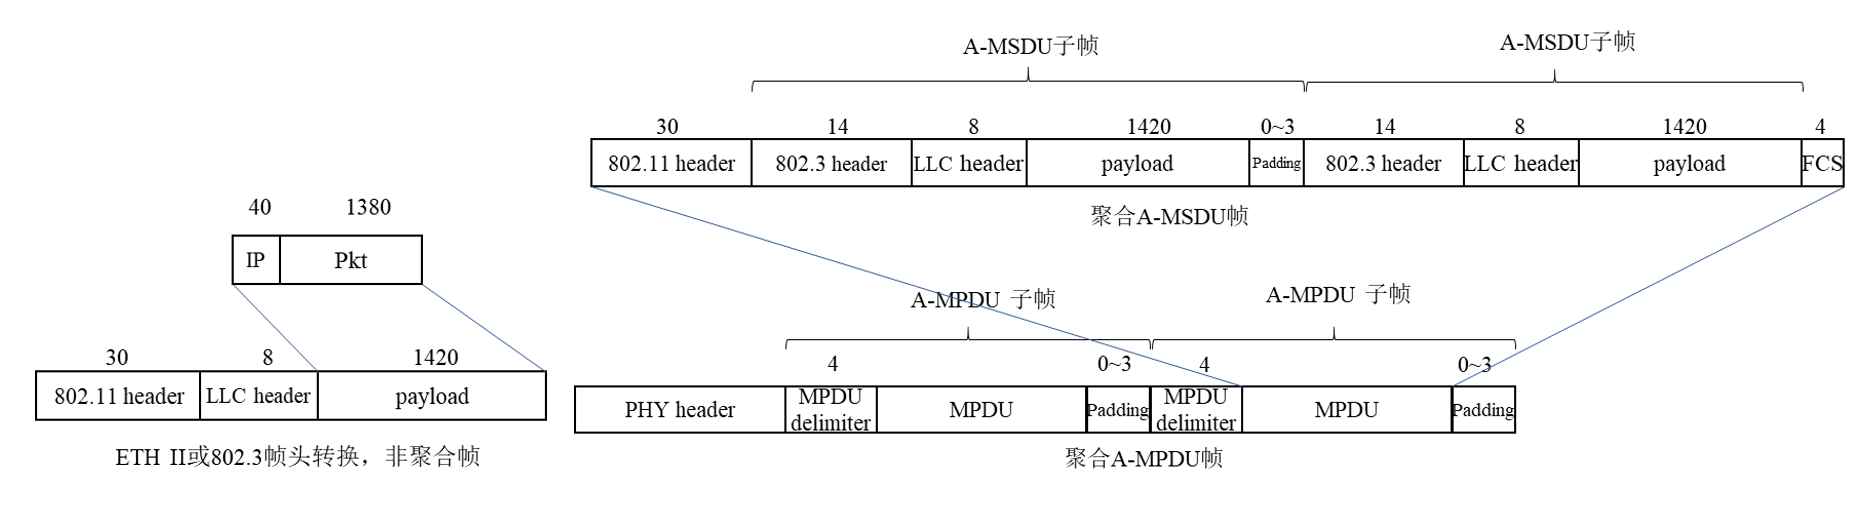
\includegraphics[scale=0.5]{juhe.png}
    \caption{\centering (a)以太网帧不聚合  (b)AMSDU聚合和AMPDU聚合}
    \label{pho:juhe}
\end{figure}
\subsection{传输方式}
当两个节点间的RSSI>ED时,一个节点传输数据时,另一节点检测信道为繁忙,称两个节点能“听”到。那么多数情况下二者的数据传输将交替进行,只在偶然同时回退到0时同时开始数据传输。节点同时发送数据时产生碰撞,可能导致传输失败。这种在节点间可侦听情况下发生的传输称为同步传输,包括交替进行和同时发生的传输。

WLAN实际部署中,受覆盖范围和可用信道数约束,工作在相同信道的同频AP间RSSI大多处于[PD, ED]区间,一个区域内同频AP数量通常为3~5个。受
业务类型影响,包长差异较大,如\ref{pho:yibu}所示,在某次同步传输过程中,先结束传输的AP2进行CCA时,由于已经错过侦听AP1的Preamble,将采用ED作
为CCA门限,从而判定信道为空闲,在回退到0时开始一次新的传输。称为异步传输。若AP1结束传输时,AP2的第二次传输已开始,则AP1同样原因可能会开始第二次传输,那么两个AP可能进入长时间的异步传输状态。

\begin{figure}[!htbp]
    \centering
    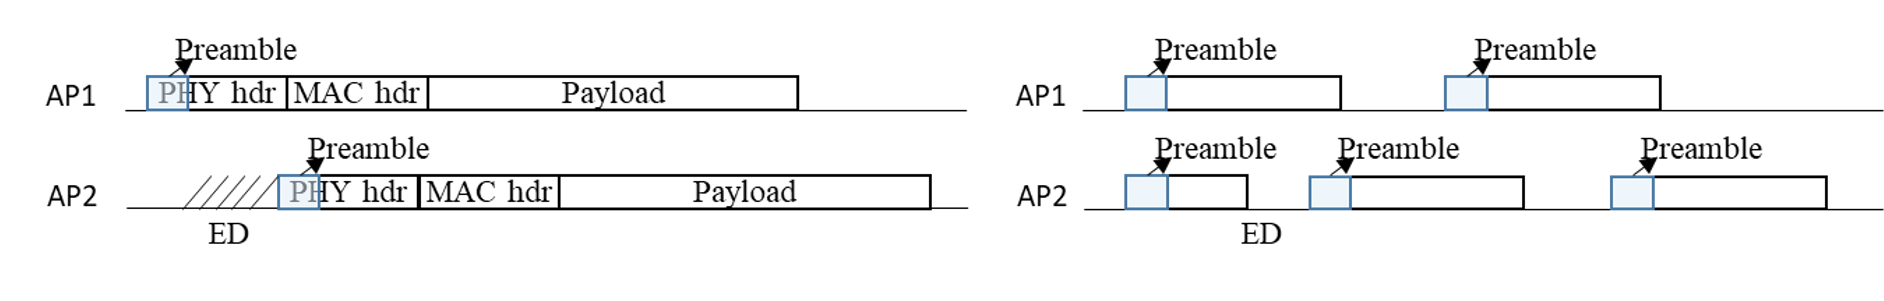
\includegraphics[scale=0.45]{yibu.png}
    \caption{\centering 一次异步传输和异步传输状态示意图}
    \label{pho:yibu}
\end{figure}
\subsection{自适应调制编码算法}
发送数据的PHY层速率(PHY Rate)由调制编码方案(Modulation and Coding Scheme, MCS)和空间流数(Number of Spatial Stream, NSS)表征,一
组(MCS, NSS)对应一个PHY Rate(见4.2节)。MCS和NSS越高,发送时携带的有效比特数越多,即PHY Rate越高。节点的PHY层对信号进行解调时,要求一定
的SINR,其SINR越高,可支持成功解调的MCS和NSS越高。WLAN采用经典的自适应调制解调(Adaptive Modulation and Coding, AMC)算法,根据信道条件
动态调整发送数据使用的(MCS, NSS)。具体地,初始化时采用默认值(如MCS6, NSS2)发送数据,并持续统计和更新丢包率(Packet Error Rate, PER)。
当PER高于一定阈值时,代表当前SINR下,以该(MCS, NSS)发送数据的解调成功率低,需要降低MCS和NSS;否则提高MCS和NSS。AMC算法自适应寻找最优的
PHY Rate发送数据,使得吞吐量最大。
\newpage
\section{问题一的分析与求解}

\subsection{问题分析}
\subsubsection{问题分析}
问题一主要研究AP发送的机会,旨在探索WLAN网络中的节点在测试场景下发送数据包的机会,即发送数据帧列的总时长(seq\_time),并构建预测模型,该问题包括两个子问题:

(1) 分析训练集中各参数对seq\_time的影响并排序:

首先,基于训练集中training\_set\_2ap\_loc0\_nav82等11个数据表,对AP=2和AP=3分类进行分析。对于每一种同频AP类型,研究表中的所提供的网络拓扑、业务流量、门限、节点间RSSI的测试基本信息,分析其中各参数对AP发送机会的影响,即对seq\_time数据值的相关性系数,并根据其影响性强弱给出重要性排序。

(2)构建模型预测每个AP的seq\_time:

根据训练集中training\_set\_2ap\_loc0\_nav82等11个数据表,分别对AP=2和AP=3构建模型预测测试集test\_set\_1\_2ap和test\_set\_1\_3ap中AP发送数据帧序列的总时长。这个模型将分别使用每一种同频AP的训练集进行训练,然后将模型应用于测试集中的AP参数,输出的seq\_time表示每个AP在一定条件下发送数据机会的大小。 

通过解决问题一的两个子问题,我们将更好地了解哪些因素能够影响AP发送数据的机会,并能够进一步研究各参数对WLAN网络吞吐量的影响。这对于无线局域网系统的进一步优化具有重要意义。

\subsubsection{求解思路}
针对上述问题,提出如下求解思路:

由题目可知,WLAN部署后,节点基于信道竞争接入机制进行CCA和随机回退,并发送数据。在节点间RSSI、信道竞争接入机制、CCA门限、NAV机制等共同影响下,节点以一定的概率发送数据。
因此,节点在某一功率下的某一时刻听到的\textbf{RSSI处于什么范围(是否超过门限)},会使得节点因此选择传输、等待(DIFS/回退)或静默,乃至导致可能的测试组内的传输方式(同步/异步),这一
机制能够很大程度上影响对节点数据帧发送时长的预测,因此除了使用训练集给定的参数外,我们还需要从这些给定数据中挖掘对应新特征表示节点状态以更好地进行预测。

\textbf{*机制分析}

通过简单观察训练集中各接收到RSSI参数的取值大小,发现其在测试中出现的可能范围于-98~-29dBm之间,结合文中提到的CCA门限以及测试中出现的两种NAV门限,
某一AP节点在某一时刻根据接入机制对信道忙闲判断如下(对RSSI取值范围):

 1. $ [ -100,NAV ) $:信道空闲。

 2. $ [ NAV,PD ) $:若未侦测到RTS,信道空闲,否则繁忙。

 3. $ [ PD,ED ) $:若未侦测到RTS,且未接收到Preamble,则信道空闲,否则信道繁忙。

 4. $ [ ED,-20 ) $:信道繁忙。
    

\begin{figure}[!htbp]
    \centering
    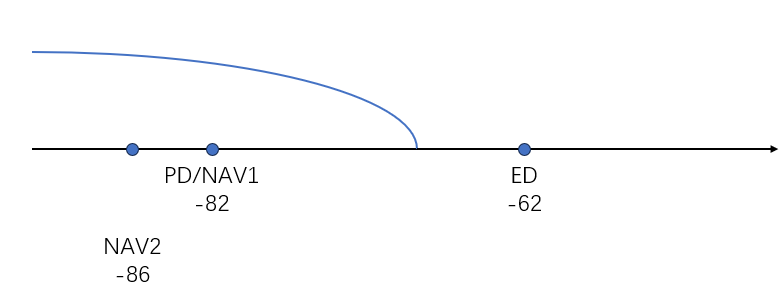
\includegraphics[scale=0.8]{menxian.png}
    \caption{\centering CCA门限、NAV门限示意图 \quad 单位(dBm)}
    \label{pho:menxian}
\end{figure}

由此机制可总结:

(1)当RSSI较小时,即其他节点信号影响较小时,AP根据对信道忙闲的判断更大可能性为空闲,并发送数据。尽管此时仍有随即回退机制的限制,但可以推断的是,此时
AP发送数据的机会更大,并导致更长的seq\_time。因此,我们可以根据对AP所听到的RSSI强弱判断,将其作为新特征变量,用于模型预测。

(2)由题可知,当两个节点间的$RSSI>ED$时,两节点互听,此时进行同步传输,每个AP交替抢到信道,偶然同时发送,发送时长基本上各占一半。当RSSI大多处于$[PD, ED]$
区间,此时进行异步传输,两个AP总是不互听时,每个AP独立持续抢到信道,发送时长基本占满,此时NAV失效。因此按照RSSI处于门限区间,将不同数据展示分类属性,
进一步推测其处的传输方法,以根据此机制预测发送时长。

为了具象化这一区间关系,我们将某一AP在一次测试中的RSSI信息数列中的每个值进行区间判断,并分别得出在测试期间RSSI处于各门限区间的概率,
具体见5.2.1(3)节。基于上述已知变量及新变量,我们将AP发送机会的计算表示为:$$asfda$$

\subsection{子问题一:各参数影响强弱分析}
\subsubsection{数据预处理}
针对所提供的网络拓扑、业务流量、门限、节点间 RSSI 的测试基本信息包括共35个可选特征变量,我们进行预处理,进行以下步骤操作。

(1)数据清洗,我们将相同同频AP个数的所有训练表合并为一个主表,对于表中观测到的异常空值,和异常数值(例如在training\_set\_3ap\_loc30\_nav86中部分列数据为空, 以及training\_set\_2ap\_loc2\_nav82最下面两行的数据与其他数据相比明显异常,数据与表头内容对不上),对此处理为删除整行数据避免对分析结果的影响。

(2)变量删除,进行部分特征变量的移除,这些变量部分是常量(即在所有数据中保持不变),部分可以以行数奇偶性为隐藏属性表示,部分只是固有属性根据经验判断与因变量seq\_time无关。删除变量包括:test\_dur、loc\_id、pkt\_len、bss\_id、ap\_name、ap\_mac、ap\_id、pd、ed、sta\_mac、sta\_id共11个变量。

(3)创建新变量。题目中提到AP传输方式对AP发送时长具有直接影响,考虑到pd,ed表现为信道传输门限,它们决定了AP的CCA机制,进而导致不同的可能传输机制,因此我们采用差值变量,以概率形式表示在某一时间点AP的传输方式可能性。变换公式如下:

(4)数据变换。对protocol变量,取01变换。对表示RSSI信息的20个变量,对数列中的各值取平均。例如:

(5)主表拆分,观测到训练数据中,每个测试由AP个数行组成,考虑到这些行之间由于在同一个测试场景中,部分RSSI数据具有互补性,将其分割为AP个数个子表,对于AP=2,按照行数对2的余数分为两个子表,对于AP=3,按照行数对3的余数分为3个子表。每个子表对应一个AP在测试中的表现。此时观察到test\_id在子表无意义,移除该变量。

(6)相关性分析,接着我们对特征变量: 协议,RSSI, nav,pro\_pd, pro\_ed等进行相关性分析(热力图)再次剔除了一些具有强线性相关的特征变量。其中主要剔除的变量是各类RSSI中的max值和mean值,因为我们认为sum值相较于前两者有更多信息,更具有代表性。

(7)子表合并,为了提升预测模型输入数据集的大小,我们将AP=2和AP=3的子表合并,形成一个新的数据集,以便于后续建模。合并过程中,对主表中互补的特征变量进行对应合并,例如,在AP=2的情境下,AP0的特征ap\_from\_ap\_1\_sum\_ant\_rssi与AP1的特征ap\_from\_ap\_0\_sum\_ant\_rssi合并为ap\_from\_ap\_other\_sum\_ant\_rssi。合并示意如图\ref{pho:hebing},具体合并规则请见附录。

\begin{figure}[!htbp]
    \centering
    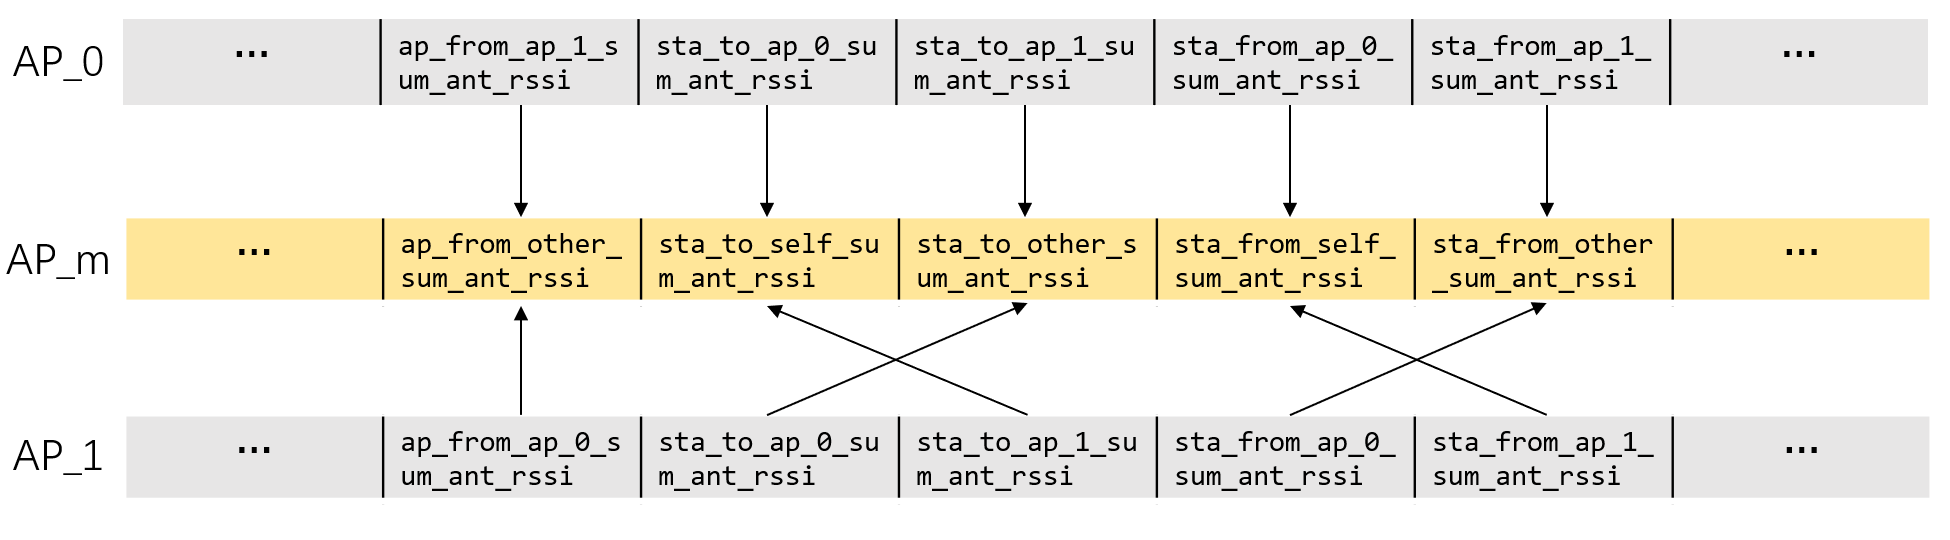
\includegraphics[scale=0.5]{hebing.png}
    \caption{\centering AP子表合并示意图}
    \label{pho:hebing}
\end{figure}
\subsubsection{模型构建}
 考虑到目标预测数据seq\_time是连续变量,并且为了充分求解特征变量对目标变量的重要性,我们采用了三种不同的建模方法:随机森林、
 XGBoost和岭回归。

 \textbf{1、随机森林(Random Forest):}
 
 随机森林是一种集成学习方法,通过随机选择特征子集训练多个决策树,最终通过投票机制得到最终结果。
 
 \textbf{2、XGBoost:}
 
 XGBoost是一种梯度提升算法,通过迭代训练多个决策树,每次训练都会根据上一次的结果调整数据的权重,最终得到最终结果。
 
 \textbf{3、岭回归(Ridge Regression):}
 
 岭回归是一种线性回归方法,通过加入正则项,可以有效防止过拟合。

 三种方法的结果(分组条形图)均显示{xxxxx}(可列表)。

 \subsection{子问题二:数据帧发送总时长预测}
 \subsubsection{模型训练}
 然后我利用上面训练出的随机森林、XGBoost、Lasso模型进行seq\_time的预测。采用交叉验证法评古模型性能。

 \textbf{1、数据集划分}

 \textbf{2、超参数选择}

 \subsubsection{模型对比}
 在进行模型训练后,我们分别对其产生的结进行交叉验证并计算出准确率,结果如表3.4所示。

 由表上表数据对比可知,随机森林模型的准确率最高,因此我们选择随机森林模型对test表进行预测。根据题目要求对测试集test\_set\_1\_2ap和test\_set\_1\_3ap中AP发送数据帧序列的总时长进行预测,并填写在对应数据位中。
 
 数学建模求解算法示例:
\begin{center}
\begin{minipage}{0.8\textwidth}
\begin{algorithm}[H]%[!htp]
\caption{算法的名字} %算法的名字
{\bf 输入:} %算法的输入, \hspace*{0.02in}用来控制位置,同时利用 \\ 进行换行
input parameters A, B, C\\
{\bf 输出:} %算法的结果输出
output result
\begin{algorithmic}[1]
\State some description 算法介绍 % \State 后写一般语句
\For{condition} % For 语句,需要和EndFor对应
  \State ...
  \If{condition} % If 语句,需要和EndIf对应
    \State ...
  \Else
    \State ...
  \EndIf
\EndFor
\While{condition} % While语句,需要和EndWhile对应
  \State ...
\EndWhile
\State \Return result
\end{algorithmic}
\end{algorithm}
\end{minipage}
\end{center}
\vspace{2ex}

\newpage
\section{问题二的分析与求解}
\subsection{问题分析}
\subsubsection{问题简述}
问题二主要研究AP在发送过程中选用的调制编码方案(Modulation and Coding Scheme, MCS)和空间流数(Number of Spatial Stream, NSS)表征。题目中要求,通过分析实测训练集中的测试基本信息,特别是节点间RSSI信息和门限信息进行分析,针对测试中AP发
送数据选用最多次数的(MCS, NSS)进行建模,使用得到的预测模型预测test\_set\_2\_2ap和test\_set\_2\_3ap中的(MCS, NSS)。

\textbf{“选用最多次数的(MCS, NSS)”}理解:经观察,训练集中每一行测试数据都给定了一组(MCS, NSS),我们认为这是AMC算法在测试初始阶段快速收敛后所得到的,并在余下的大部分测试期间都使用这一组(MCS, NSS)用于解调信号,即选用最多次数的(MCS, NSS)。

通过得到这一数值对(MCS, NSS),可以一定程度上表示AP发送数据的PHY层速率(PHY Rate),其可以作为求解第三问系统吞吐量的前置影响条件。

\subsubsection{求解思路}
针对上述问题,提出如下求解思路:

由题目可知,AP发送数据时的PHY层速率PHY Rate取决于调制编码方案MCS和空间流数NSS,而这两者(MCS, NSS)又由信号解调时的SINR决定。WLAN采用AMC自适应调制解调算法,平衡当前SINR下所支持的(MCS, NSS)数值大小,以保证丢包率不高于一定阈值。因此,处理本题时,需要通过测试信息,初步计算信道SINR信息,以进一步预测对应的(MCS, NSS)。

AP的AMC所选用的(MCS, NSS)不仅与SINR相关,同时也与AP的传输方式相关。可以总结的,两个AP之间的传输方式有三种可能:同步传输、异步传输、同步异步混合传输。在各个传输方式下,因为STA接收数据时受到的干扰来源不同,导致SINR的计算方法也不同。因此,为了计算信道SINR信息,需要确定各测试数据所处的传输方式,而这一过程需结合问题一中使用节点间RSSI信息和门限信息进行分类的方法。

综上所述,为解决问题二,我们首先根据节点间RSSI信息和门限信息对其所处\textbf{传输方式}进行分类,随后根据其实际传输方式用不同的计算方式得到对应\textbf{SINR信息},进一步地,利用SINR对\textbf{(MCS, NSS)}数值进行预测。
\subsubsection{机制分析}
分析各节点之间的RSSI信息和门限信息,可以得出在WLAN信道争夺机制下,AP可能处于如下三种传输方式:

\textbf{(1)同步传输:}此时AP间RSSI>PD且RSSI>NAV,两AP之间互听,交替抢到信道,偶然同时发送,且NAV生效。STA接受数据时干扰主要来自环境底噪,此时SINR计算如下:

\textbf{(2)异步传输:}此时AP间RSSI<PD且RSSI<NAV,两AP之间不互听,邻区干扰小,同时进行数据发送,NAV不生效。此时STA接收数据时可能受到较小的邻区干扰和环境底噪,因此,SINR计算如下:

\textbf{(3)同步与异步传输混合:}此时两个AP的RSSI>PD且RSSI<NAV,两AP之间互听,邻区干扰大,NAV不生效。当传输中出现由于错过Preamble时,无法利用NAV更新通知其他AP,导致异步传输。此时STA接收数据时受到的干扰根据具体处于的传输方式决定,SINR计算如下:

根据各节点间RSSI信息处于门限区间,计算得出对应SINR值,以预测对应的(MCS, NSS)。
\subsection{问题求解}
\subsubsection{数据处理}
在第一问处理的基础上,本问题进一步确定了因为AP间RSSI所处门限区间,用以分类其在一次测试中的主要传输方式,以此进一步计算SINR数值。

通过上题的数据处理,我们创建了3个新的特征值(在3AP情况是两组共6个):pro\_pd、pro\_ed、pro\_nav,分别表示了某AP在一次测试期间接收到来自其他
组内AP的RSSI高于PD、ED、NAV门限的频率,以此近似表示在以此次传输中各测量时刻该AP根据接受到的RSSI数值进行判断,进而进行对应接入操作的概率。
由于新特征呈现连续性,取值处于$[0,1]$之间,且具有不均匀性,为了在进行门限区间分类时使用准确的阈值,我们采用K-means聚类辅助分析。
K-means介绍:

聚类结果如上图。
创建新的特征变量'SINR',根据分类类型,使用6.1.3节提到的计算方法分别计算对应SINR值。
\subsubsection{模型构建}
\subsubsection{结果分析}

\newpage
\section{问题三的分析与求解}
\subsection{问题分析}
\subsubsection{问题简述}
问题三主要研究WLAN网络系统吞吐量预测。题目要求结合问题一和问题二的分析,利用前两问的预测指标,包括AP发送数据帧序列的总时长、(MCS, NSS)以及其他测试基本信息,共同构建预测模型,通过测试集test\_set\_1\_2ap和test\_set\_1\_3ap预测网络吞吐量。其中问题二所预测得到的(MCS, NSS)无法获得很高精度,允许采用实测中统计的数据帧真实(MCS, NSS)作为模型输入变量。

问题三是本课题的最终研究目标,前两问通过分析WLAN网络拓扑、节点间RSSI、信道接入机制、干扰等因素对WLAN数据发送、速率的影响,本问题进一步地利用其预测结果作为重要影响因素与支撑,对WLAN系统吞吐量进行精确预测。基于该吞吐量预测模型,对WLAN进行优化,有望突破工业、教育、医疗等新场景,为用户提供极致的业务体验。
\subsubsection{求解思路}
根据题目背景,给出如下定义:
\begin{itemize}
    \item 吞吐量:吞吐量指节点单位时间内成功发送的比特数。仅MSDU的总字节数是有效传输数据,进行吞吐量计算。
    \item 丢包率:发送数据帧的失败个数与总个数的百分比。
    \item 数据的帧序列的总时长:所有成功或失败的数据帧发送,帧序列时长从开始发送RTS到收到ACK,或者超时。
    \item ppdu\_dur (s):一个数据帧的时长。一次测试里,统计每个数据帧的时长,取平均值。仅包括PPDU的传输时间,不包括RTS,ACK等。
    \item TCP的ACK算是数据帧,算作吞吐量,个数是下行数据帧的3:1到2:1左右。根据丢包率改变传输速率。TCP ACK的大小为64Bytes。
    \item UDP仅计算AP发往STA的数据帧,发送时间间隔服从泊松分布,发送数据的速率为290 Mbps。
\end{itemize}



根据题目可知,WLAN网络吞吐量主要取决于AP发送机会、发送时所选用的PHY Rate以及数据帧的比特数。

\textbf{(1)数据包聚合计算:}

为了提升发送小包的效率,协议允许通过聚合一次发送多个具有相同目的地址的数据包。在一次数据包聚合(AMSDU)过程中,多个相同接收地址的同服务类别的MAC服务数据单元(MSDU)封装成一个MAC协议数据单元(MPDU)。组装好的多个MPDU进一步聚合(AMPDU),这一过程包括将多个MPDU聚合成一个PHY协议数据单元(PPDU)。此处PPDU即为在WLAN网络中进行传输的一个数据帧。

其中,组成MPDU的MSDU包长计算如式\ref{eq:msdu}(单位:Bytes):
\begin{align}
    MSDU &= 802.3\text{header} + LLC\text{header} + \text{payload} + \text{padding} \nonumber\\
         &= 14 + 8 + 1500 + 2 \label{eq:msdu} \\
         &= 1524\nonumber
    \end{align}
    
其中,组成PPDU的MPDU包长计算如式\ref{eq:mpdu}(单位:Bytes):
\begin{align}
    MPDU &= 802.11header + MSDU \times AMSDU - \text{padding} + FCS \nonumber\\
         &= 30 + 1524 \times AMSDU - 2 + 4 \label{eq:mpdu}\\
         &= 32 + 1524 \times AMSDU \nonumber
    \end{align}
    
最终,计算一个完整数据帧PPDU的包长(在WLAN协议(如802.11标准)中,**PHY头(Physical Layer Header)**的长度取决于
所使用的物理层(PHY)类型,不是固定的。不同的PHY模式会有不同的PHY头大小。)(单位:Bytes)式\ref{eq:ppdu}:
\begin{align}
    PPDU &= (4 + MPDU + \text{padding}) \times AMPDU + PHY(\text{长度不固定}) \label{eq:ppdu}
    \end{align}
    

\subsection{问题求解}
\subsubsection{数据预处理}
\subsubsection{模型构建}
\subsubsection{结果分析}

\section{表格和图形}

\subsection{表格}

%\begin{table}[!htbp]
%    \caption{标准三线表格}\label{tab:001} \centering
%    \begin{tabular}{ccccc}
%        \toprule%[1.5pt]
%        $D$(in) & $P_u$(lbs) & $u_u$(in) & $\beta$ & $G_f$(psi.in)\\
%        \midrule%[1pt]
%        5 & 269.8 & 0.000674 & 1.79 & 0.04089\\
%        10 & 421.0 & 0.001035 & 3.59 & 0.04089\\
%        20 & 640.2 & 0.001565 & 7.18 & 0.04089\\
%        \bottomrule%[1.5pt]
%    \end{tabular}
%\end{table}

三线表

%\begin{table}[!htp]
%\renewcommand\arraystretch{1.0} %定义表格高度
%\newcolumntype{L}{X}
%\newcolumntype{C}{>{\centering \arraybackslash}X}
%\newcolumntype{R}{>{\raggedright \arraybackslash}X}
%\centering
%\caption{某校学生升高体重样本}
%\label{tab2:heightweight}
%\begin{tabularx}{0.9\textwidth}{CC|CC}
%   \toprule
%	\multicolumn{2}{c}{Numbers} &身高&体重\\
%	\midrule
%	1&14&156&42\\
%	2&16&158&45\\
%	3&14&162&48\\
%	4&15&163&50\\
%    \midrule
%    %\cmidrule{2-4}
%	平均&15&159.75&46.25\\
%	\bottomrule
%\end{tabularx}
%\end{table}



\begin{table}[!htp]
\renewcommand\arraystretch{1.0} %定义表格高度
\newcolumntype{L}{X}
\newcolumntype{C}{>{\centering \arraybackslash}X}
\newcolumntype{R}{>{\raggedright \arraybackslash}X}
\centering
\caption{某校学生升高体重样本}
\label{tab2:heightweight}
\begin{tabularx}{0.9\textwidth}{|C|C|C|C|}
   \Xhline{2\arrayrulewidth}
	\multicolumn{2}{|c|}{Numbers}  &身高&体重\\
	\Xhline{2\arrayrulewidth}
	\multirow{2}{*}{Item} &14&156&42\\
    \cline{2-4}
	  &16&158&45\\
    \hline
	3&14&162&48\\
    \hline
	4&15&163&50\\
    %\cmidrule{2-4}
	平均&15&159.75&46.25\\
	\Xhline{2\arrayrulewidth}
\end{tabularx}
\end{table}


题目要求建立模型描述折叠桌的动态变化图,由于在折叠时用力大小的不同,我们不能描述在某一时刻折叠桌的具体形态,但我们可以用每根木条的角度变化来描述折叠桌的动态变化。首先,我们知道折叠桌前后左右对称,我们可以运用几何知识求出四分之一木条的角度变化。最后,根据初始时刻和最终形态两种状态求出桌腿木条开槽的长度。题目要求建立模型描述折叠桌的动态变化图,由于在折叠时用力大小的不同,我们不能描述在某一时刻折叠桌的具体形态,但我们可以用每根木条的角度变化来描述折叠桌的动态变化。首先,我们知道折叠桌前后左右对称,我们可以运用几何知识求出四分之一木条的角度变化。最后,根据初始时刻和最终形态两种状态求出桌腿木条开槽的长度。题目要求建立模型描述折叠桌的动态变化图,由于在折叠时用力大小的不同,我们不能描述在某一时刻折叠桌的具体形态,但我们可以用每根木条的角度变化来描述折叠桌的动态变化。首先,我们知道折叠桌前后左右对称,我们可以运用几何知识求出四分之一木条的角度变化。最后,根据初始时刻和最终形态两种状态求出桌腿木条开槽的长度题目要求建立模型描述折叠桌的动态变化图,由于在折叠时用力大小的不同,我们不能描述在某一时刻折叠桌的具体形态,但我们可以用每根木条的角度变化来描述折叠桌的动态变化。首先,我们知道折叠桌前后左右对称,我们可以运用几何知识求出四分之一木条的角度变化。最后,根据初始时刻和最终形态两种状态求出桌腿木条开槽的长度

某行业产量与生产费用的数据
\begin{table}[htp!]
\centering
\caption{某行业产量与生产费用的数据}%\label{}
\newcolumntype{Y}{>{\centering\arraybackslash}X}
\newcolumntype{Z}{!{\vline}@{\color{white}\vrule width \doublerulesep}!{\vrule}}%自定义列格式(双线)
\begin{tabularx}{0.94\textwidth}{c|c|YZc|c|Y}
    \Xhline{0.9pt}
	企业编号&	产量(台)&生产费用(万元)&企业编号&产量(台)&生产费用(万元)\\
    \Xcline{1-3}{0.6pt}\Xcline{4-6}{0.6pt}
	1&	40&	130&7&	84&	165\\
	2&	42&	150&8&	100&	170\\
	3&	50&	155&9&	116&	167\\
	4&	55&	140&10&	125&	180\\
	5&	65&	150&11&	130&	175\\
	6&	78&	154&12&	140&	185\\
    \Xhline{0.72pt}
\end{tabularx}
\end{table}

研究生数学建模2019年F题结果示例

\begin{table}[htp!]
    \centering
    \caption{问题1结果1 (左) 与 问题2结果 (右)}
    \renewcommand\arraystretch{1.2} %定义表格高度
    \newcolumntype{Y}{>{\centering\arraybackslash}X}
    \begin{tabularx}{0.9\textwidth}{|Y|Y|Y|}
      \hline
      数据集1  &  数据集1 & 数据集2  \\
     \hline
      AP\_0   & AP\_1 &  AP\_merge    \\
      \hline
      503   &  503     & 163     \\
      294   &  200     & 114      \\
      91    &  80      & 8     \\
      607   &  237     & 309      \\
      540   &  170     & 305    \\
      250   &  278     & 123    \\
      340   &  369     & 45      \\
      277   &  214     & 160    \\
      B     &  397     & 92    \\
            &  B       & 93    \\
            &          & 61        \\
            &          & 292       \\
            &          & B         \\
    104861  & 103518   & 109342 \\
    \hline
    \end{tabularx}
    \end{table}


    \begin{table}[htp!]
        \centering
        \caption{2AP子表变量合并}
        \begin{tabular}{|l|l|l|l|}
            \hline
              & AP\_0                            & AP\_1                            & AP\_merge                        \\
            \hline
            0 & protocol                         & protocol                         & protocol                         \\
            1 & nav                              & nav                              & nav                              \\
            2 & ap\_from\_ap\_1\_sum\_ant\_rssi  & ap\_from\_ap\_0\_sum\_ant\_rssi  & ap\_from\_other\_sum\_ant\_rssi  \\
            3 & sta\_to\_ap\_0\_sum\_ant\_rssi   & sta\_to\_ap\_1\_sum\_ant\_rssi   & sta\_to\_self\_sum\_ant\_rssi    \\
            4 & sta\_to\_ap\_1\_sum\_ant\_rssi   & sta\_to\_ap\_0\_sum\_ant\_rssi   & sta\_to\_other\_sum\_ant\_rssi   \\
            5 & sta\_from\_ap\_0\_sum\_ant\_rssi & sta\_from\_ap\_1\_sum\_ant\_rssi & sta\_from\_self\_sum\_ant\_rssi  \\
            6 & sta\_from\_ap\_1\_sum\_ant\_rssi & sta\_from\_ap\_0\_sum\_ant\_rssi & sta\_from\_other\_sum\_ant\_rssi \\
            7 & pro\_pd                          & pro\_pd                          & pro\_pd                          \\
            8 & pro\_ed                          & pro\_ed                          & pro\_ed                          \\
            9 & pro\_nav                         & pro\_nav                         & pro\_nav                         \\
            \hline
        \end{tabular}
    \end{table}

\begin{table}[htp!]
\centering
\caption{问题1结果1 (左) 与 问题2结果 (右)}
\begin{minipage}[h]{0.48\linewidth}
\renewcommand\arraystretch{1.2} %定义表格高度
\newcolumntype{Y}{>{\centering\arraybackslash}X}
\begin{tabularx}{0.9\textwidth}{|Y|Y|Y|}
  \hline
  数据集1  &  数据集1 & 数据集2  \\
 \hline
  A问题1   & A问题1 &  A问题1     \\
  \hline
  503   &  503     & 163     \\
  294   &  200     & 114      \\
  91    &  80      & 8     \\
  607   &  237     & 309      \\
  540   &  170     & 305    \\
  250   &  278     & 123    \\
  340   &  369     & 45      \\
  277   &  214     & 160    \\
  B     &  397     & 92    \\
        &  B       & 93    \\
        &          & 61        \\
        &          & 292       \\
        &          & B         \\
104861  & 103518   & 109342 \\
\hline
\end{tabularx}
\end{minipage}
\begin{minipage}[h]{0.48\linewidth}
\renewcommand\arraystretch{1.2} %定义表格高度
\newcolumntype{Y}{>{\centering\arraybackslash}X}
\begin{tabularx}{0.9\textwidth}{|Y|Y|Y|}
  \hline
  数据集1  &  数据集1 & 数据集2  \\
  \hline
  A问题2  &  A问题2  & A问题2    \\
  \hline
   503    & 503     & 163  \\
  294    & 200     & 114   \\
   91     & 80     & 8   \\
   607    & 237     & 309   \\
   540    & 170    & 305  \\
   250    & 278    & 123  \\
   340    & 369     & 45   \\
   277    & 214    & 160  \\
  B      & 397   & 92 \\
        &  B     &  93      \\
         &         &  61      \\
        &         &   292     \\
        &         &   B     \\
 104917  &  103563  &109427 \\
\hline
\end{tabularx}
\end{minipage}
\end{table}

\clearpage
\begin{table}[htp!]
%\small
\centering
\renewcommand\arraystretch{1.2} %定义表格高度
\newcolumntype{Y}{>{\centering\arraybackslash}X}
\caption{问题3结果}
\begin{tabularx}{0.9\textwidth}{|Y|Y|Y|Y|Y|Y|}
  \hline %定义表格宽度
  数据集1  &  数据集1  &  \multicolumn{2}{c|}{数据集2 (无问题点)}  & \multicolumn{2}{c|}{数据集2 (有问题点)} \\
  \hline
  A问题3   & A问题3   &  \multicolumn{2}{c|}{A问题3}    &  \multicolumn{2}{c|}{A问题3}      \\
  \hline
  503      & 503     & 169      & 73      & 169     & 73   \\
  \hline
  69       & 69      & 322      & 249     & 322     & 249   \\
  \hline
  506      & 506      & 270     & 274     & 270     & 274   \\
  \hline
  371      & 371      & 89      & 12      & 89      & 12   \\
  \hline
  183      & 183      & 236     & 216     & 236     & 216  \\
  \hline
  194      & 194      & 132     & 16      & 132     & 16   \\
  \hline
  450      & 450      & 53      & 282     & 53      & 282   \\
  \hline
  286      & 113      & 112     & 84      & 112     & 141  \\
  \hline
  485      & 485      &  268    & 287     & 268     & 291 \\
  \hline
 \red{B (9D)}~~     & 248      & 250     & 99      & 250     &161 \\
 \hline
   & \red{B (10D)}   & 243     & \red{B (21D)}   & 243    & \red{B (21D)} \\
   \hline
    &          &         &         &         &       \\
    \hline
  104861m  & 103518m  &         & 168924m  &         &161650m \\
\hline
\end{tabularx}
\end{table}


\subsection{图形}

图形并列
\begin{figure}[htp!]
\begin{minipage}[t]{0.48\linewidth}
\centering
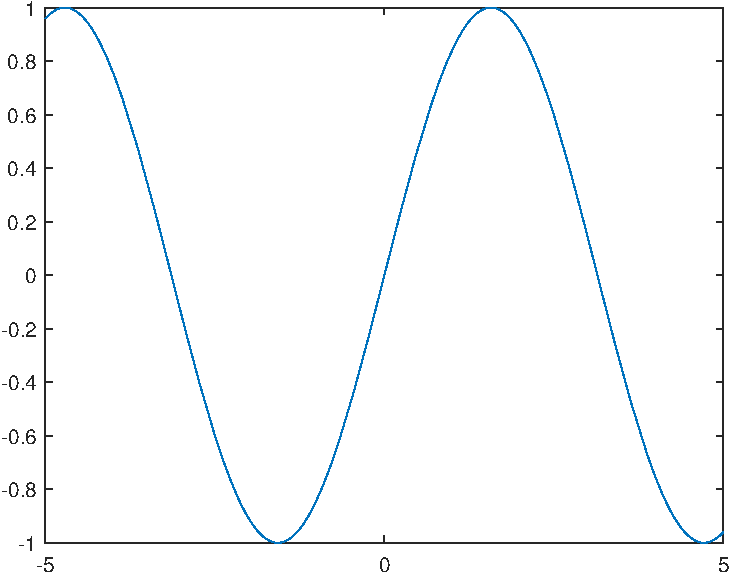
\includegraphics[width=0.9\textwidth]{image1}
\caption{fig1}
\label{fig:side:a}
\end{minipage}%
\begin{minipage}[t]{0.48\linewidth}
\centering
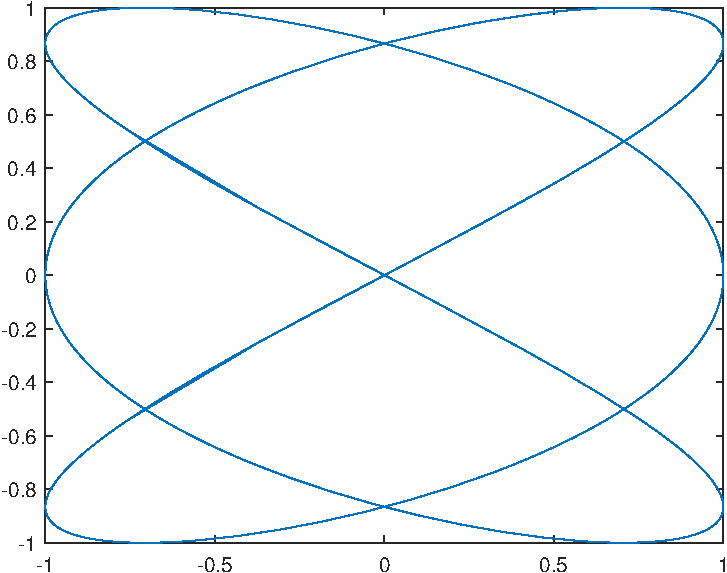
\includegraphics[width=0.9\textwidth]{image2}  % 2.2in
\caption{fig2}
\label{fig:side:b}
\end{minipage}
\end{figure}

这是一个算法流程图
\begin{figure}[htp!]
\centering
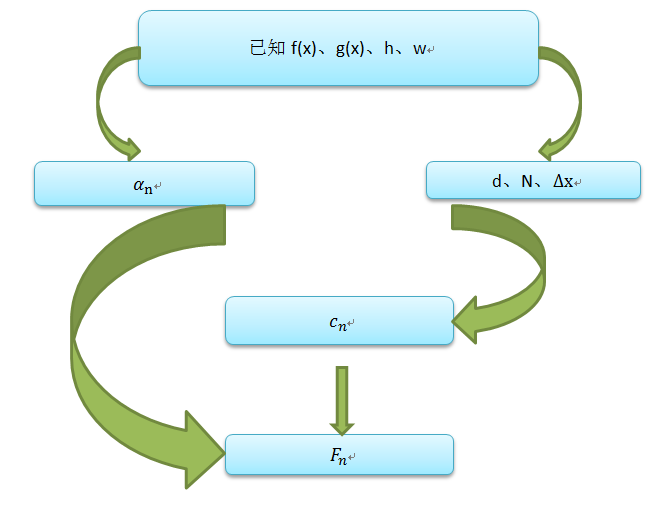
\includegraphics[width=.55\textwidth]{fig.png}
\caption{算法流程图}
\end{figure}

多图并排
\begin{figure}[!htp]
	\centering
	\subfloat[Arabic numerals]{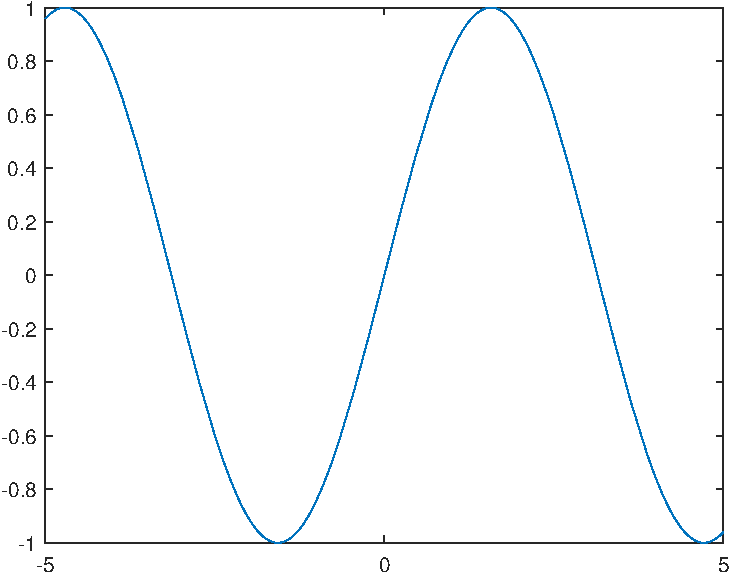
\includegraphics[width=0.4\textwidth]{image1}}\qquad
	\subfloat[Arabic numerals]{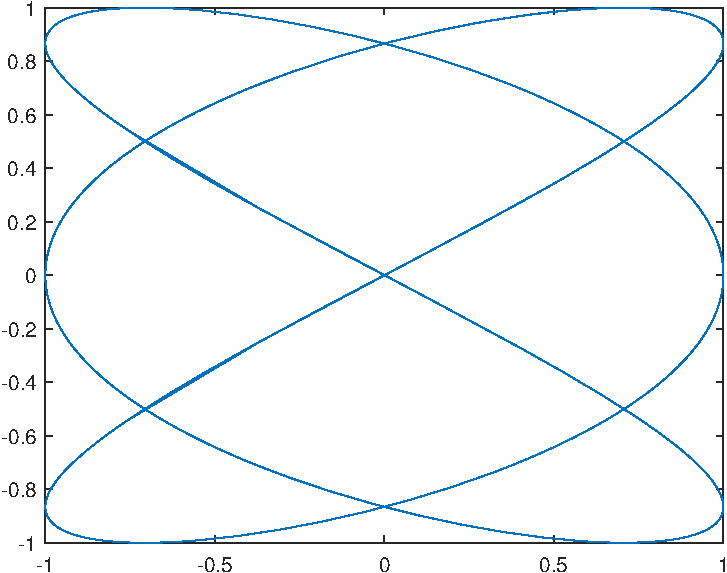
\includegraphics[width=0.4\textwidth]{image2}} \\
	\subfloat[Arabic numerals]{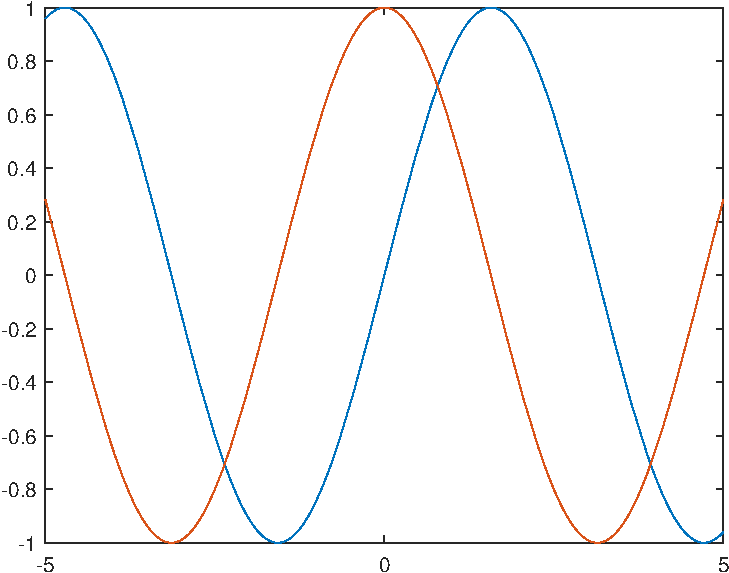
\includegraphics[width=0.4\textwidth]{image3}}\qquad
	\subfloat[Arabic numerals]{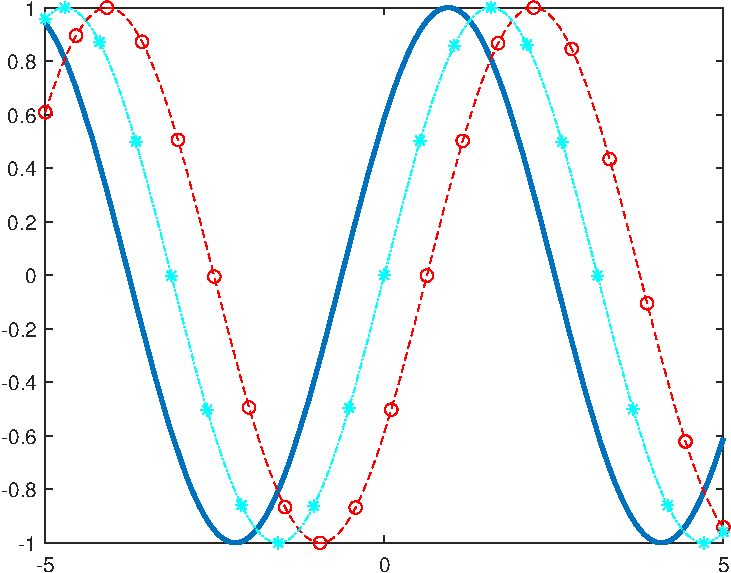
\includegraphics[width=0.4\textwidth]{image4}}
	\caption{多图示例}
\end{figure}


\clearpage
\subsection{问题三分析}

题目要求制作软件的意思就是客户给定折叠桌高度、桌面边缘线的形状大小和桌脚边缘线的大致形状,将这些信息输入程序就得到客户想要的桌子。我们在求解最优设计加工参数时,自行给定桌面边缘线形状(椭圆、相交圆等),桌脚边缘线形状,折叠桌高度,应用第二问的非线性规划模型,用MATLAB软件绘制折叠桌截面图,得到自己设计的创意平板折叠桌。


\section{模型评价}

这里是模型评价



%参考文献   手工录入
%\begin{thebibliography}{9}%宽度9
% \bibitem{bib:one} ....
% \bibitem{bib:two} ....
%\end{thebibliography}

%采用bibtex方案
\cite{mittelbach_latex_2004,wright_latex3_2009,beeton_unicode_2008,vieth_experiences_2009,ls:2024}

\bibliographystyle{gmcm}
\bibliography{reference}


\clearpage
%附录
\begin{appendices}
%\setcounter{page}{1} %如果需要可以自行重置页码。
\section{MATLAB 源程序}
\renewcommand{\thesubsection}{A\thinskip.\thinskip\arabic{subsection}}
\subsection{第1问程序}
\vspace{-2ex}

\begin{Matlab}{code.m}
clear all
kk=2;
[mdd,ndd]=size(dd);
while ~isempty(V)
    [tmpd,j]=min(W(i,V));
    tmpj=V(j);
    for k=2:ndd
        [tmp1,jj]=min(dd(1,k)+W(dd(2,k),V));
        tmp2=V(jj);
        tt(k-1,:)=[tmp1,tmp2,jj];
    end
    tmp=[tmpd,tmpj,j;tt];
    [tmp3,tmp4]=min(tmp(:,1));
    if tmp3==tmpd,
        ss(1:2,kk)=[i;tmp(tmp4,2)];
    else
        tmp5=find(ss(:,tmp4)~=0);
        tmp6=length(tmp5);
        if dd(2,tmp4)==ss(tmp6,tmp4)
            ss(1:tmp6+1,kk)=[ss(tmp5,tmp4);tmp(tmp4,2)];
        else, ss(1:3,kk)=[i;dd(2,tmp4);tmp(tmp4,2)];
        end
    end
    dd=[dd,[tmp3;tmp(tmp4,2)]];
    V(tmp(tmp4,3))=[];
    [mdd,ndd]=size(dd);kk=kk+1;
end;
S=ss; D=dd(1,:);
\end{Matlab}
\vspace{2ex}

\clearpage
\section{Python 源程序}
\renewcommand{\thesubsection}{B\thinskip.\thinskip\arabic{subsection}}
\subsection{第2问程序}
\vspace{-2ex}
\begin{Python}{mip1.py}
# This example formulates and solves the following  MIP model:
#  maximize
#        x +   y + 2 z
#  subject to
#        x + 2 y + 3 z <= 4
#        x +   y       >= 1
#        x, y, z binary

# import gurobipy as gp
from gurobipy import * #GRB
try:
    # Create a new model
    m = Model("mip1")
    # Create variables
    x = m.addVar(vtype=GRB.BINARY, name="x")
    y = m.addVar(vtype=GRB.BINARY, name="y")
    z = m.addVar(vtype=GRB.BINARY, name="z")
    # Set objective
    m.setObjective(x + y + 2 * z, GRB.MAXIMIZE)
    # Add constraint: x + 2 y + 3 z <= 4
    m.addConstr(x + 2 * y + 3 * z <= 4, "c0")
    # Add constraint: x + y >= 1
    m.addConstr(x + y >= 1, "c1")
    # Optimize model
    m.optimize()
    for v in m.getVars():
        print('%s %g' % (v.varName, v.x))
    print('Obj: %g' % m.objVal)

except GurobiError as e:
    print('Error code ' + str(e.errno) + ': ' + str(e))

except AttributeError:
    print('Encountered an attribute error')
\end{Python}

\end{appendices}



\end{document} 